\documentclass[10pt]{article}
%\usepackage[margin=1.5in]{geometry}
\usepackage{amsmath}
\usepackage{amsfonts}
\usepackage{amssymb}
\usepackage{graphicx}
\usepackage{natbib}

\title{Inside Outside Recursive Neural Network for\\
Unsupervised Compositional Semantics Learning}
\author{Phong Le}

\begin{document}

\maketitle

%%%%%%%%%%%%%%%%%%%%%%%%%%%%%%%%%%%%%%%%%%
\section{Introduction}
\label{section introduction}

There are many reasons why distributional \textit{lexical} semantics has become popular in 
computational linguistics. Firstly, it has strong support from not only linguistics but
also cognitive science \citep{lenci_distributional_2008}. Secondly, that kind of semantics 
can be \textit{learned} 
from unannotated data, which are redundant and free on the Internet, thanks to 
the flourish of unsupervised learning techniques, such as  Latent semantic analysis 
\citep{landauer1998introduction}, neural network 
language modelling \citep{collobert_natural_2011, huang2012improving}, Brown clustering
algorithm \citep{brown1992class}, and 
spectral learning \citep{dhillon2012two}. And finally, it has many applications such as 
in information retrieval, sentiment analysis, and syntactic parsing.

However, its sister, distributional \textit{compositional} semantics, is still very 
challenging since available techniques for distributional lexical semantics are not 
applicable. The core problem lies in the the sparsity of data: there are not enough 
data (and I believe that we will never be able to collect enough data) since the number 
of semantically plausible phrases is infinitive. In this report, I will firstly point out  
hypotheses that are used in many approaches in order to solve the challenge, in Section~
\ref{section hypotheses}. Then, I will propose a new framework, namely Inside 
Outside Recursive Neural Network (IORNN), in Section~\ref{section iornn}, and Dialogue Context 
Inside Outside Recursive Neural Network (DC-IORNN), in Section~\ref{section dciornn}. 
In Section~\ref{section applications}, I will point out three important applications for that framework.

%%%%%%%%%%%%%%%%%%%%%%%%%%%%%%%%%%%%%%%%%%
\section{Hypotheses}
\label{section hypotheses}
The \textit{distributional hypothesis} states that \citep{lenci_distributional_2008}
\begin{quote}
The degree of semantic similarity between two linguistic expressions A and B is a function
of the similarity of the linguistic contexts in which A and B can appear. 
\end{quote}
This hypothesis can be rewritten, in machine learning terms, for lexical semantics learning as follows
\begin{quote}
\textit{Hypothesis 1:} The agreement between words and contexts provides enough 
evidence for lexical semantics learning.
\end{quote}
and for phrasal semantics learning as follows
\begin{quote}
\textit{Hypothesis 2:} The agreement between phrases and contexts provides enough evidence
for phrasal semantics learning.
\end{quote}

Unfortunately, it turns out that the hypothesis 2 is useless if it stands alone: we will never collect 
enough data for learning since the number of well-grammatical phrases is infinitive. Hence, 
people looked for another direction, which relies on the \textit{principle of compositionality} 
\citep{partee_lexical_1995}
\begin{quote}
The meaning of a complex expression is a function of the meaning of its parts and of the syntactic
rules by which they are combined. 
\end{quote}
However, the principle itself doesn't point out how to construct compositionality functions, 
which are the target of many research on distributional compositional semantics. 

The most simple approach is use vector addition and multiplication as compositionality functions
\citep{mitchell_vector-based_2008}. Those functions, although no parameters need to be optimized, 
are too simple to capture real compositionality. 

Socher and colleagues propose two neural network frameworks: recursive auto encoder (RAE) 
\citep{socher_semi-supervised_2011}, (and latter, unfolding RAE \citep{socher_dynamic_2011}) for 
unsupervised learning, and recursive neural network for supervised learning with task-based 
training signal \citep{socher_learning_2010}
(e.g., for sentiment analysis, the training signal is the sentiment given by voters)
(and later, MV-RNN \citep{socher_semantic_2012} and RNTN \citep{socher2013recursive}). 
The key idea of the RAE framework is that: a compositionality function is a compression function, 
such that an input is able to be recovered from the output by a decompression function. 
In other words, the following hypothesis is used 
\begin{quote}
\textit{Hypothesis 3:} Phrases themselves, along with their syntactic structures, 
provide enough evidence for distributional compositional 
semantics learning.
\end{quote}
%However, in reality, this hypothesis could not be true. For instance, `fake gun' is not a true gun, 
%but a thing \textit{looks} similar to a gun. 

\cite{baroni_frege_2012}, \cite{grefenstette_multi-step_2013} and others attempt the challenge 
in a different way. 
They use tensors to represent functor words (i.e., verbs, adjectives, etc.), 
linear maps as compositionality functions, and use contexts for estimating tensors' elements and 
functions' parameters. Hence, we can say that those approaches make use of Hypothesis 2. 
Those approaches, although relying on the principle of compositionality, also suffer 
the sparsity of data because there are too many parameters to optimize. 

From those approaches, we can see that there are three main key factors for a successful 
approach: (i) the expressiveness of compositionality functions, (ii) the ability to overcome 
the sparsity of data, and (iii), the most important one, the strength of training signal. 

In this report, I propose a new framework based on the following hypothesis
\begin{quote}
\textit{Hypothesis 4:} The agreement between words and contexts provides enough evidence
for compositional semantics learning. 
\end{quote}
(Note the difference between Hypothesis 4 and Hypothesis 1.) The key idea here is that, 
compositionality functions are used for composing the meanings of contexts, under the 
constraint that those meanings are able to be used to predict the target words. This 
comes from the observation that a human being can guess the meaning of an unknown
word given a context around it. In order to do that, he must use the meaning of the context
to infer the meaning of the word. Therefore, if he successfully infers the meaning of that
word, we can say that, at some degree of certainty, he comprehends the context. 

There are three important points. Firstly, although many of those approaches also make use 
of context, they rely on the `flat' relationship between words and contexts, which is stored in
\textit{co-occurrence} matrices. My framework, in contrast, focuses on the meaning 
of context and how to construct it. Hence, it can capture stronger constraints between 
words and contexts and make use of data better in order to overcome the problem of 
sparsity of data.

Secondly, what my framework gives to a phrase is not only its meaning without context
but also the meaning of its context (we call them \textit{inner meaning} and 
\textit{outer meaning} respectively).
Hence, when combining the two kinds of meaning, 
we can come up with phrasal semantics in context, which is important in information
retrieval \citep{korkontzelos2013semeval}. In addition, we can also compute the 
semantic plausibility of a phrase in a specific context, which is useful for syntactic parsing
\citep{lazaridou2013fish}.

Finally, my framework is general in the sense that, it can make use of 
any neural net framework proposed by Socher and colleagues. For the RAE framework, 
the training signal 
is now even stronger since it uses not only phrases and their syntactic structures but also the 
agreement between words and contexts. For the RNN framework, we now can train RNNs 
in an unsupervised learning manner. 
This framework, therefore, possesses those three key factors.

%%%%%%%%%%%%%%%%%%%%%%%%%%%%%%%%%%%%%%%%%%
\section{Inside Outside Recursive Neural Network (IO-RNN)}
\label{section iornn}
In this section, I will present my framework. In order to be simple, RNN is used. 
However, as I mentioned before, any networks which can process tree structures 
are also applicable. 

\subsection{Network Structure}
\begin{figure}[h!]
	\center
	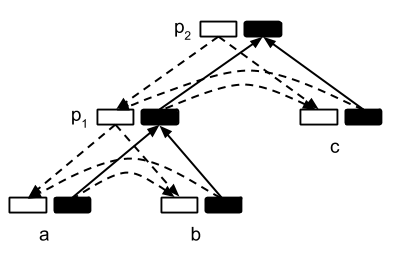
\includegraphics[scale=0.5]{IO-RNN.png}
	\caption{Inside-Outside Recursive Neural Network. Black rectangles correspond to inner meanings, 
	white rectangles correspond to outer meanings.}
	\label{figure iornn}
\end{figure}

Given a constituent and its tree structure (like the one in Figure~\ref{figure iornn}), 
each node $u$ is assigned two vectors $\mathbf{o}_u$ and $\mathbf{i}_u$. The first one,
called \textit{outer meaning}, denotes the meaning of the context; the second one, 
called \textit{inner meaning}, denotes the meaning of the phrase that the node covers.

\paragraph{Word embeddings} (e.g., $\mathbf{i}_a$)
Similar to \cite{socher_learning_2010}, and \cite{collobert_natural_2011}, given a string of binary
representations of words $(a, b, ..., w)$ (i.e., all of the entries of $w$ are zero except the one 
corresponding to the index of the word in the dictionary), 
we first compute a string of vectors $(\mathbf{i}_{a},...,\mathbf{i}_{w})$ 
representing inner meanings of those words by using 
a look-up table (i.e., word embeddings) $\mathbf{L} \in \mathbb{R}^{n \times |V|}$, 
where $|V|$ is the size of the vocabulary and $n$ is the dimensionality of the vectors. 
This look-up table $\mathbf{L}$ could be seen as a storage of lexical semantics where each column 
is a vector representation of a word. Hence, 
\begin{equation}
    \label{equation compute word vector}
    \mathbf{i}_{w} = \mathbf{L} w \in \mathbb{R}^n
\end{equation}

\paragraph{Computing inner meaning} The inner meaning of a non-terminal node, say $p_1$, is given by
\begin{equation}
	\mathbf{i}_{p_1} = f(\mathbf{W}_1^i \mathbf{i}_{a} + \mathbf{W}_2^i \mathbf{i}_{b} + \mathbf{b}^i)
	\label{equation inner}
\end{equation}
where $\mathbf{W}_1^i, \mathbf{W}_2^i$ are $n \times n$ real matrices, 
$\mathbf{b}^i$ is a bias vector, and $f(.)$ is an activation function, e.g. $tanh$ 
function. Intuitively, the inner meaning of a parent node is the function of the inner meanings 
of its children. This is similar to what \cite{socher_learning_2010} call recursive neural network.

\paragraph{Computing outer meaning} The outer meaning of the root node, $\mathbf{o}_{root}$, is initially 
set randomly, and then learnt later. To a node which is not the root, say $p_1$, the outer meaning is given by
\begin{equation}
	\mathbf{o}_{p_1} = g(\mathbf{W}_1^o \mathbf{o}_{p_2} + \mathbf{W}_2^o \mathbf{i}_{c} + \mathbf{b}^o)
	\label{equation outer}
\end{equation}
where $\mathbf{W}_1^o, \mathbf{W}_2^o$ are $n \times n$ real matrices, 
$\mathbf{b}^o$ is a bias vector, and $g(.)$ is an activation function, e.g. $tanh$ 
function. Informally speaking, the outer meaning of a node (i.e., the meaning of 
its context) is the function of the outer meaning of its parent and the inner meaning 
of its sister. 

The reader, if familiar with syntactic parsing, could recognizes the similarity between 
Equation~\ref{equation inner}, ~\ref{equation outer}
and the inner, outer probabilities given a parse tree
\begin{equation}
	P_{in}(A,r,t) = P(A \rightarrow B\;C) P_{in}(B,r,s) P_{in}(C,s,t)
\end{equation}
\begin{equation}
	P_{out}(B,r,s) = P(A \rightarrow B\;C) P_{out}(A,r,t) P_{in}(C,s,t)
\end{equation}
Therefore, I name the framework Inside-Outside Recursive Neural Network.

\subsection{Learning}
The learning is based on the Hypothesis 4. That is there must be a strong correlation 
between $\mathbf{o}_{w}$ and $\mathbf{i}_{w}$ where $w$ is any word in 
a given sentence. The simplest way to train the network is to force 
$\mathbf{o}_{w_j} = \mathbf{i}_{w_j}$; hence, learning is to minimize the following 
loss function
\begin{equation}
	J(\theta) = \sum_{s \in D} \sum_{w \in s} \| \mathbf{o}_{w} - \mathbf{i}_{w} \|
\end{equation}
where $D$ is a set of training sentences and $\theta$ are the network parameters. 
However, that could be problematic because 
the meaning of context is not necessary the meaning of the target word.

Here, based on the observation that the meaning of context sets constraints on 
selecting a word to fill in the blank, I put a \textit{softmax} neuron unit on the top 
of each $\mathbf{o}_w$ in order to predict what $w$ is
\begin{equation}
	\hat{w} = softmax(\mathbf{W}^l \mathbf{o}_w + \mathbf{b}^l)
\end{equation}
where $\mathbf{W}^l$ is a $n \times |V|$ matrix, and 
\begin{equation}
	softmax((z_1,...,z_n)^T) = \frac{1}{\sum_j e^{z_j}} \big( e^{z_1},..., e^{z_n} \big)^T
\end{equation}
And therefore, the loss function needs to be minimized is a cross entropy loss function 
\begin{equation}
	J(\theta) = \sum_{s \in D} \sum_{w \in s} \sum_j -w_j log(\hat{w}_j)
\end{equation}
Intuitively, the loss function computes the word prediction error of the net over all 
words of all training sentences. 
The gradient $\frac{\partial J}{\partial \theta}$ could be effectively computed 
thanks to backpropagation through the structure \citep{goller_learning_1996}.


%%%%%%%%%%%%%%%%%%%%%%%%%%%%%%%%%%%%%%%%%%
\section{IO-RNN with Dialogue Context (DC-IO-RNN)}
\label{section dciornn}
It turns out that is is easy to extend the framework above to dialogue context, and 
I call the new framework DC-IO-RNN.
Figure~\ref{figure dciornn} illustrates how to connect inner and outer meanings 
of sentences in a dialogue. Intuitively, the outer meaning of a sentence is 
the function of the inner meanings of its neighbour sentences. 

\begin{figure}[h!]
	\center
	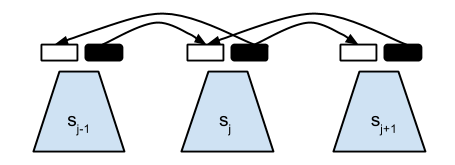
\includegraphics[scale=0.5]{DC-IO-RNN.png}
	\caption{Inside-Outside Recursive Neural Network with Dialogue Context. 
	Black rectangles correspond to inner meanings, 
	white rectangles correspond to outer meanings.}
	\label{figure dciornn}
\end{figure}

%%%%%%%%%%%%%%%%%%%%%%%%%%%%%%%%%%%%%%%%%%
\section{Applications}
\label{section applications}

\subsection{Syntactic Parsing}
\cite{lazaridou2013fish} point out that \textit{semantic plausibility} is useful for discriminating 
correct from incorrect syntactic structures. The question is what could be used to compute 
semantic plausibility. Here, I believe that the agreement between inner meaning and outer meaning
could be used as a measure for that. And therefore, we can make use of reranker methods, 
such as ones proposed by \cite{socher2013parsing} and \cite{le2013learning}.

\subsection{Word Meaning in Context}
Current research on word meaning in context \citep{huang2012improving,
thater2011word, dinu2010measuring, erk2008structured, dinu2012comparison}
focuses on `flat' relations of  target words
and their context, e.g. relations of target words and individual neighbour words. 
In contrast, my framework computes the meaning of context and hence we can 
make use of the fact that context words interact with each other in order to shift the 
meaning of the target word.

\subsection{Sentiment Analysis}
\cite{socher2012semantic} conclude that pretraining (in a unsupervised learning manner)
a MV-RNN does not help to improve the final performance on sentiment analysis 
since ``antonyms often get similar vectors [...] due to high similarity of 
local syntactic contexts''. That is true if sentences are processed independently. 
However, if all sentences in a dialogue or paragraph are processed at the same time
by DC-IO-RNN (see Section~\ref{section dciornn}), antonyms could be well 
distinguishable. The reason is that, in a positive/negative paragraph, positive/negative words tend
to occur together, though in different sentences, and DC-IO-RNN is hopfully able to capture that.

\subsection{Paraphrasing}
[???]

\subsection{Dialogue Modeling with DC-IO-RNN}
[???]



\bibliographystyle{apalike}
\bibliography{ref}

\end{document}
